\documentclass[aspectratio=169]{beamer}

% ── UOC brand colours ──
\definecolor{darkblueUOC}{RGB}{1,0,115}
\definecolor{lightblueUOC}{RGB}{147,234,252}
\definecolor{airblueUOC}{RGB}{92,138,168}
\definecolor{greyUOC}{RGB}{239,239,239}

% ── Theme setup (inspired by LDV template) ──
\usetheme{default}
\useinnertheme{default}
\usefonttheme{serif}
\usepackage{times}
\setbeamertemplate{navigation symbols}{}

% ── Colours ──
\setbeamercolor{structure}{fg=darkblueUOC}
\setbeamercolor{normal text}{fg=black, bg=white}
\setbeamercolor{frametitle}{fg=darkblueUOC, bg=white}
\setbeamercolor{title}{fg=darkblueUOC}
\setbeamercolor{subtitle}{fg=airblueUOC}
\setbeamercolor{author}{fg=darkblueUOC}
\setbeamercolor{institute}{fg=airblueUOC}
\setbeamercolor{date}{fg=airblueUOC}
\setbeamercolor{local structure}{fg=airblueUOC}
\setbeamercolor{item}{fg=airblueUOC}
\setbeamercolor{block title}{bg=greyUOC, fg=darkblueUOC}
\setbeamercolor{block body}{bg=greyUOC!50!white, fg=black}
\setbeamercolor{block title alerted}{bg=red!20, fg=black}
\setbeamercolor{block body alerted}{bg=red!10, fg=black}
\setbeamercolor{block title example}{bg=lightblueUOC!50, fg=darkblueUOC}
\setbeamercolor{block body example}{bg=lightblueUOC!20, fg=black}

% ── Fonts (LDV style: small title, large frametitle) ──
\setbeamerfont{title}{size=\large, series=\bfseries}
\setbeamerfont{subtitle}{size=\normalsize}
\setbeamerfont{author}{size=\normalsize}
\setbeamerfont{institute}{size=\scriptsize}
\setbeamerfont{date}{size=\scriptsize}
\setbeamerfont{frametitle}{size=\large, series=\bfseries}
\setbeamerfont{framesubtitle}{size=\footnotesize}
\setbeamerfont{block title}{size=\normalsize, series=\bfseries}
\setbeamerfont{item}{size=\normalsize}
\setbeamerfont{footnote}{size=\tiny}

% ── Header: UOC logo, no line ──
\setbeamertemplate{headline}{
  \vspace{0.2cm}
  \hfill
\includegraphics[height=0.8cm]{UOCllarg.png}\hspace{0.5cm}
  \par\vspace{0.1cm}
}

% ── Footer: Slide N/M only, no line ──
\setbeamertemplate{footline}{
  \vspace{2pt}
  \hfill\textcolor{airblueUOC}{\scriptsize Slide \insertframenumber/\inserttotalframenumber}\hspace{0.5cm}
  \vspace{4pt}
}

% ── Frame title with section number ──
\setbeamertemplate{frametitle}{
  \vspace{0.3em}
  \usebeamerfont{frametitle}\usebeamercolor[fg]{frametitle}\insertframetitle
  \par\vspace{-0.2em}
}

\usepackage{graphicx}
\usepackage{booktabs}
\usepackage{eurosym}
\usepackage{multirow}
\usepackage{hyperref}
\usepackage{tabularx}

\title{Demand Forecasting for Inventory Management Using Machine Learning}
\subtitle{\vspace{0.5em} Master in Data Science}
\author{Ona Mas i Serra}
\institute{
  Universitat Oberta de Catalunya\\[0.3em]
  Supervisor: Lorena Polo Navarro\\
  PRA: Susana Acedo Nadal
}
\date{June 2026}
\titlegraphic{
\includegraphics[height=1.5cm]{UOCllarg.png}}

\begin{document}

% ══════════════════════════════════════════════════════════════
% TITLE
% ══════════════════════════════════════════════════════════════
{
\setbeamertemplate{headline}{}
\setbeamertemplate{footline}{}
\setbeamercolor{subtitle}{fg=darkblueUOC}
\setbeamercolor{institute}{fg=black}
\setbeamercolor{date}{fg=black}
\begin{frame}[noframenumbering]
\titlepage
\end{frame}
}

% ══════════════════════════════════════════════════════════════
% OUTLINE
% ══════════════════════════════════════════════════════════════
\begin{frame}{Outline}
\begin{columns}[T]
\begin{column}{0.48\textwidth}
\begin{enumerate}
    \item Introduction
    \item Data
    \item Methodology
    \item Results
\end{enumerate}
\end{column}
\begin{column}{0.48\textwidth}
\begin{enumerate}
    \setcounter{enumi}{4}
    \item Interpretability
    \item Economic Impact
    \item Conclusions
\end{enumerate}
\end{column}
\end{columns}
\end{frame}

% ══════════════════════════════════════════════════════════════
% 1. INTRODUCTION
% ══════════════════════════════════════════════════════════════
\section{Introduction}

\begin{frame}{1. Introduction: Context}
\begin{itemize}
    \item Demand forecasting is critical for inventory management in the automotive sector
    \item Inaccurate forecasts lead to excess stock (capital tied up) or stockouts (lost sales, production disruptions)
    \item Safety stock acts as a buffer against demand uncertainty
    \item More accurate forecasts = less safety stock needed = lower costs
\end{itemize}
\vfill
\begin{block}{Safety stock formula}
Safety stock is directly proportional to forecast error: $SS = z \times RMSE \times \sqrt{T + L}$
\end{block}
\end{frame}

\begin{frame}{1. Introduction: Objectives}
\begin{enumerate}
    \item Conduct a bibliographic review of demand forecasting methods
    \item Explore and prepare a real automotive sector dataset
    \item Implement and compare multiple forecasting models
    \item Evaluate promotional vs non-promotional demand
    \item Compare all models against a naive baseline
    \item Quantify the economic impact on safety stock costs
\end{enumerate}
\end{frame}

% ══════════════════════════════════════════════════════════════
% 2. DATA
% ══════════════════════════════════════════════════════════════
\section{Data}

\begin{frame}{2. Data: Dataset Overview}
\begin{columns}
\begin{column}{0.5\textwidth}
\begin{itemize}
    \item Real data from an automotive company
    \item 861 products, 731 days
    \item March 2024 to March 2026
    \item 629,391 daily observations
    \item 65.3\% zero-sales observations
    \item Fully anonymised
\end{itemize}
\end{column}
\begin{column}{0.5\textwidth}
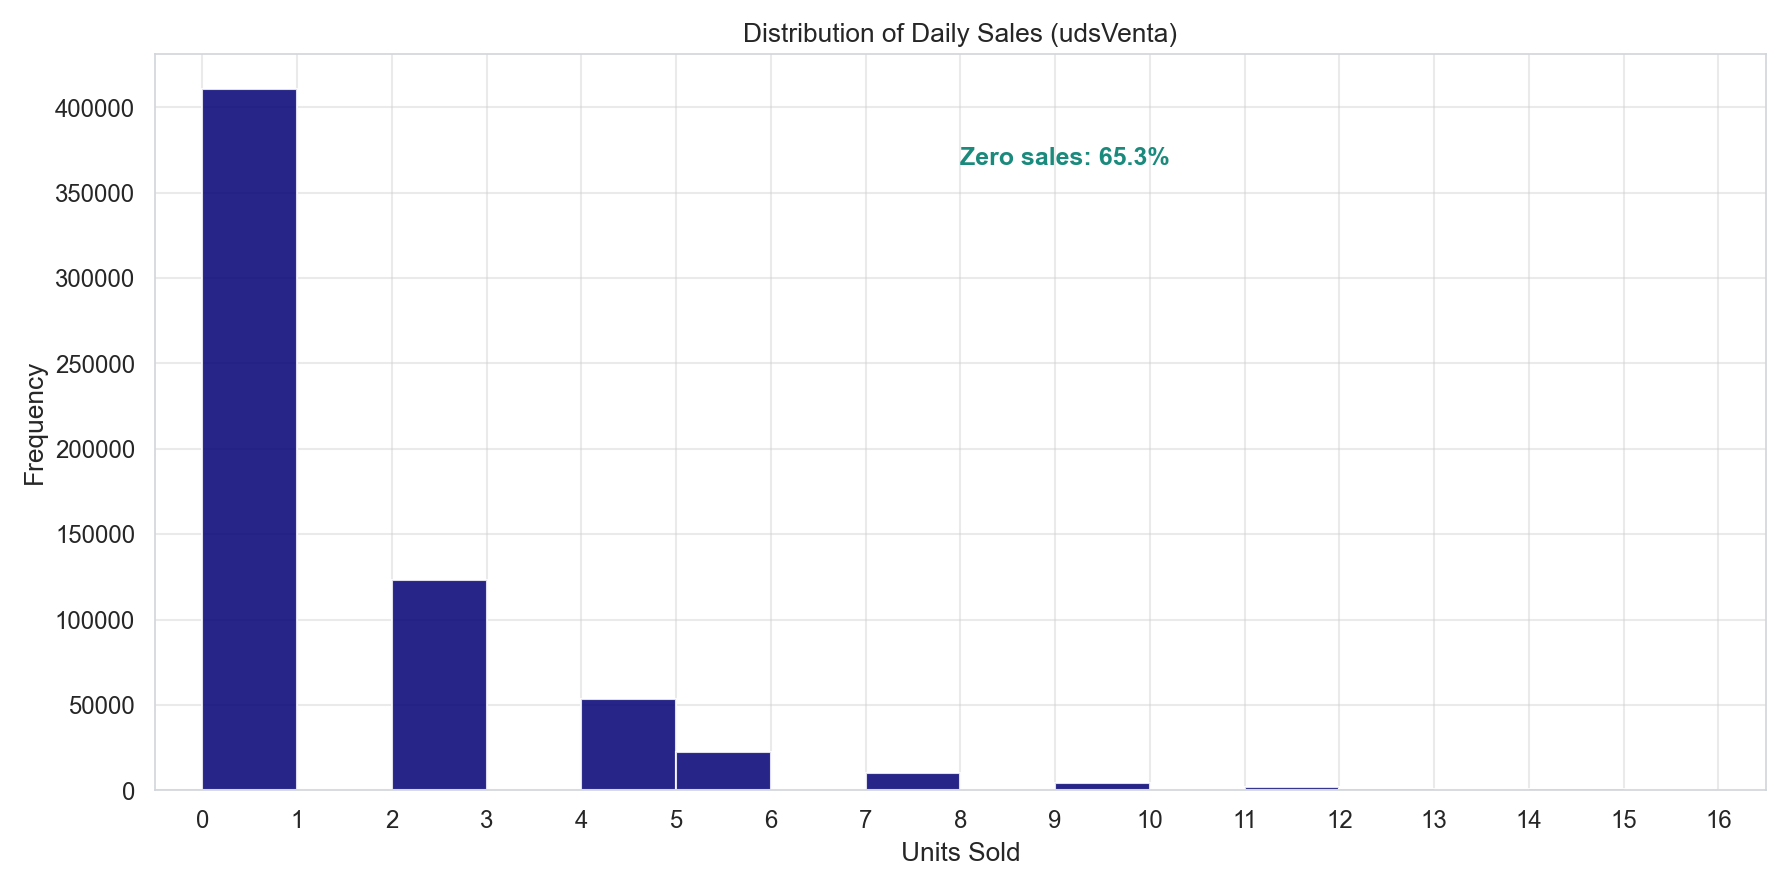
\includegraphics[width=\textwidth]{figures/01_sales_distribution.png}
\end{column}
\end{columns}
\end{frame}

\begin{frame}{2. Data: Demand Patterns}
\begin{columns}
\begin{column}{0.5\textwidth}
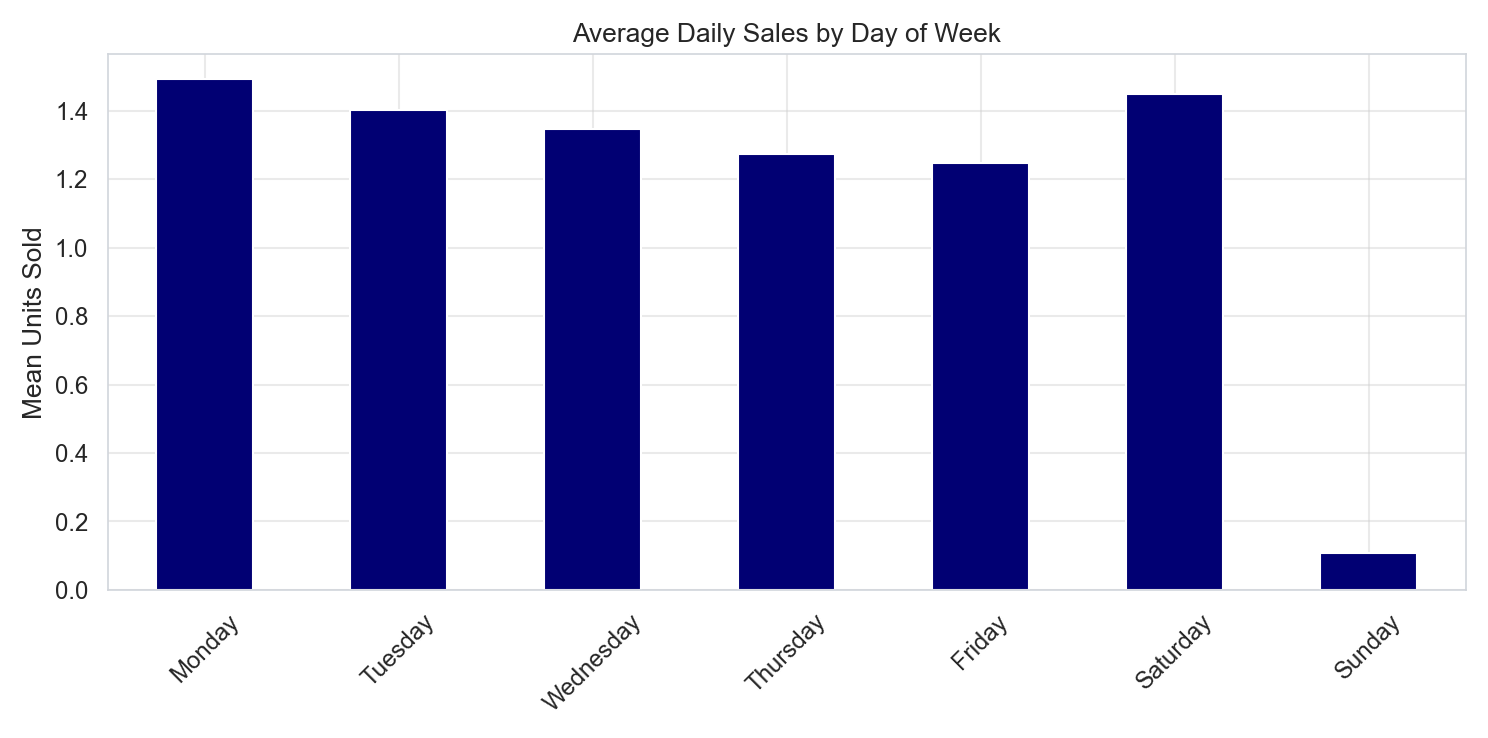
\includegraphics[width=\textwidth]{figures/02_sales_by_day_of_week.png}
\end{column}
\begin{column}{0.5\textwidth}
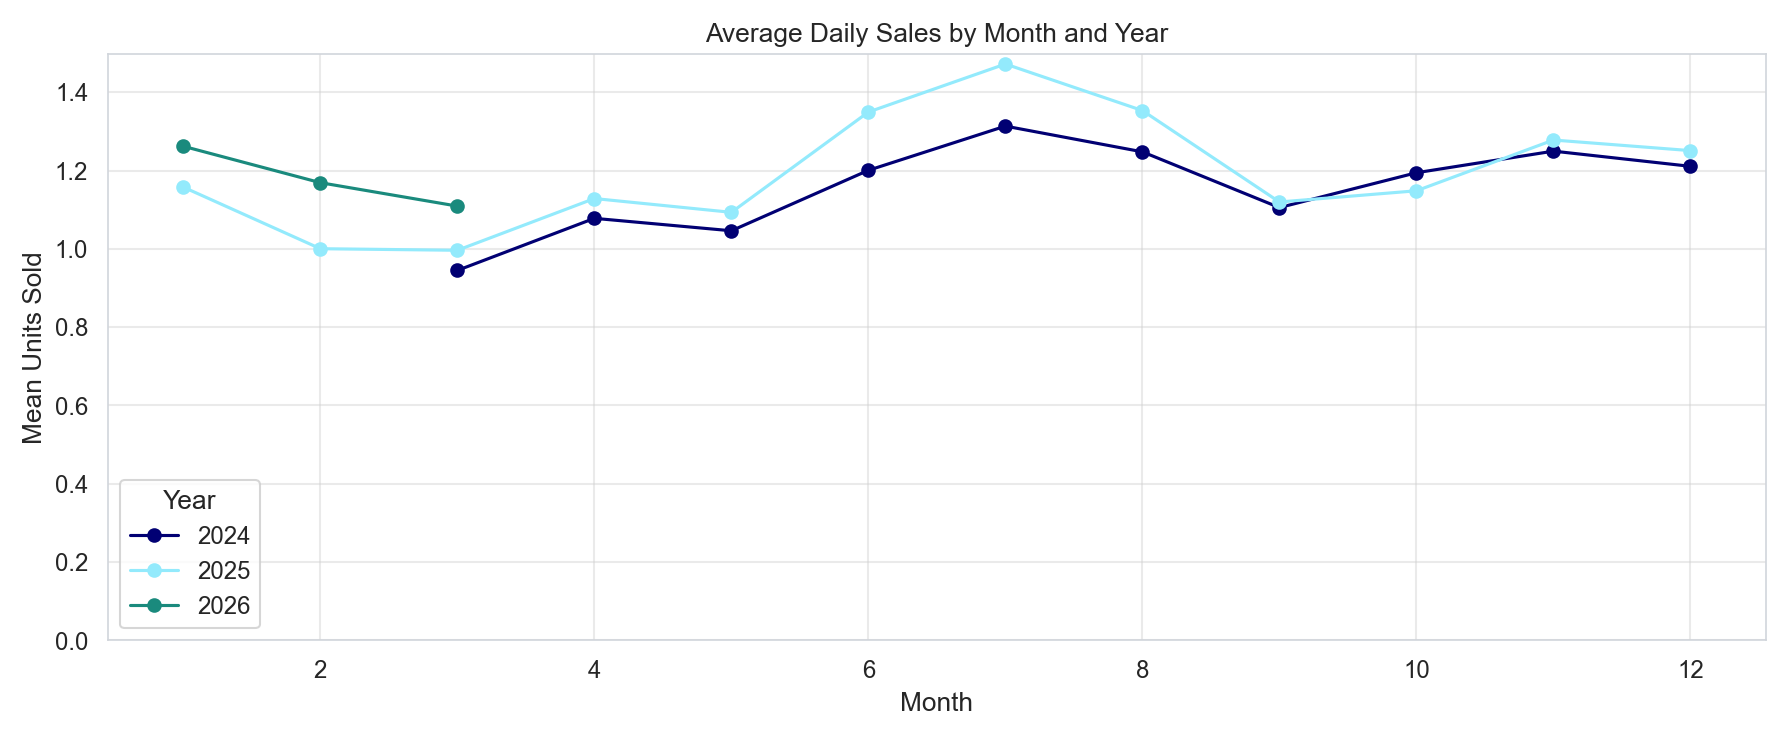
\includegraphics[width=\textwidth]{figures/09_monthly_by_year.png}
\end{column}
\end{columns}
\vfill
\begin{itemize}
    \item Consistent demand Monday through Saturday, near-zero on Sundays
    \item Moderate monthly variation, no dominant seasonal peak
    \item Strong weekly autocorrelation at lag 7 (motivates naive baseline)
\end{itemize}
\end{frame}

% ══════════════════════════════════════════════════════════════
% 3. METHODOLOGY
% ══════════════════════════════════════════════════════════════
\section{Methodology}

\begin{frame}{3. Methodology: Pipeline}
\begin{table}
\centering
\small
\begin{tabular}{clp{7cm}}
\toprule
\textbf{Step} & \textbf{Phase} & \textbf{Description} \\
\midrule
1 & EDA & Exploratory analysis of demand patterns \\
2 & Preprocessing & Stock break imputation (2\%), outlier capping (1.4\%) \\
3 & Feature Engineering & 33 features: calendar, lags, rolling stats, EWMA, promotional \\
4 & Modelling & 6 models trained with rolling validation (3 folds, 30 days) \\
5 & Evaluation & Accuracy metrics, SHAP interpretability, error analysis \\
6 & Economic Impact & Safety stock cost comparison using real company data \\
\bottomrule
\end{tabular}
\end{table}
\vfill
\begin{itemize}
    \item CRISP-DM methodology
    \item Hyperparameter tuning with Optuna (30 trials per model)
\end{itemize}
\end{frame}

\begin{frame}{3. Methodology: Models}
\begin{table}
\centering
\small
\begin{tabular}{ll}
\toprule
\textbf{Model} & \textbf{Type} \\
\midrule
Naive (lag-7) & Baseline (same weekday last week) \\
ARIMA (Seasonal) & Classical time series (per product) \\
Random Forest & Tree ensemble (bagging) \\
XGBoost & Gradient boosting \\
LightGBM & Gradient boosting (histogram-based) \\
LSTM & Deep learning (recurrent neural network) \\
\bottomrule
\end{tabular}
\end{table}
\vfill
\begin{itemize}
    \item Tree-based models: hyperparameters tuned with Optuna (30 trials each)
    \item ARIMA: auto\_arima with weekly seasonality ($m=7$), fitted to all 861 products
    \item LSTM: single layer (32 units), 14-day input sequences, PyTorch
\end{itemize}
\end{frame}

% ══════════════════════════════════════════════════════════════
% 4. RESULTS
% ══════════════════════════════════════════════════════════════
\section{Results}

\begin{frame}{4. Results: Forecast Accuracy}
\begin{table}
\centering
\small
\begin{tabular}{lrrrr}
\toprule
\textbf{Model} & \textbf{MAE} & \textbf{RMSE} & \textbf{MAPE} & \textbf{$\sigma_e$} \\
\midrule
LightGBM & 1.097 & 1.633 & 51.5\% & 1.633 \\
XGBoost & 1.121 & 1.635 & 50.0\% & 1.634 \\
Random Forest & 1.098 & 1.637 & 50.0\% & 1.636 \\
LSTM & 1.148 & 1.662 & 49.6\% & 1.655 \\
ARIMA & 1.211 & 1.734 & 53.9\% & 1.732 \\
Naive (lag-7) & 1.256 & 2.277 & 74.4\% & 2.277 \\
\bottomrule
\end{tabular}
\end{table}
\vfill
\begin{itemize}
    \item Three tree-based models achieve virtually identical performance
    \item All ML models reduce RMSE by 24--28\% vs naive baseline
    \item RMSE directly enters the safety stock formula
\end{itemize}
\end{frame}

\begin{frame}{4. Results: Model Comparison}
\begin{center}
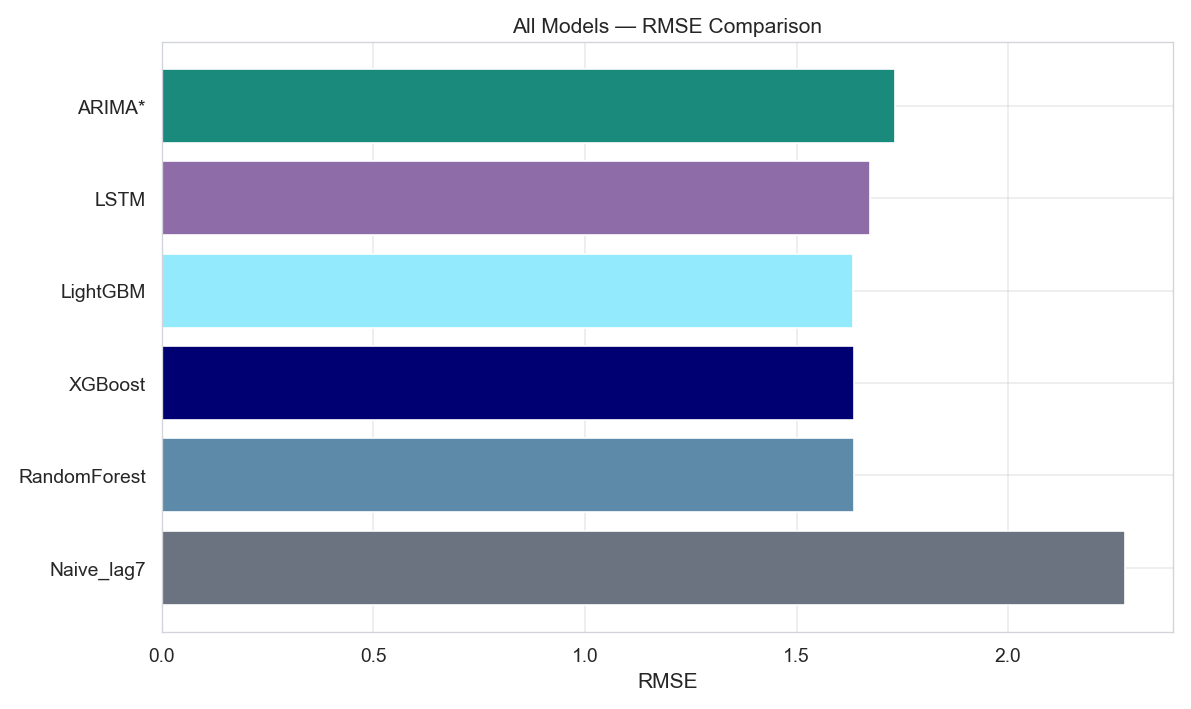
\includegraphics[width=0.75\textwidth]{figures/24_all_models_comparison.png}
\end{center}
\end{frame}

\begin{frame}{4. Results: Error Analysis}
\begin{center}
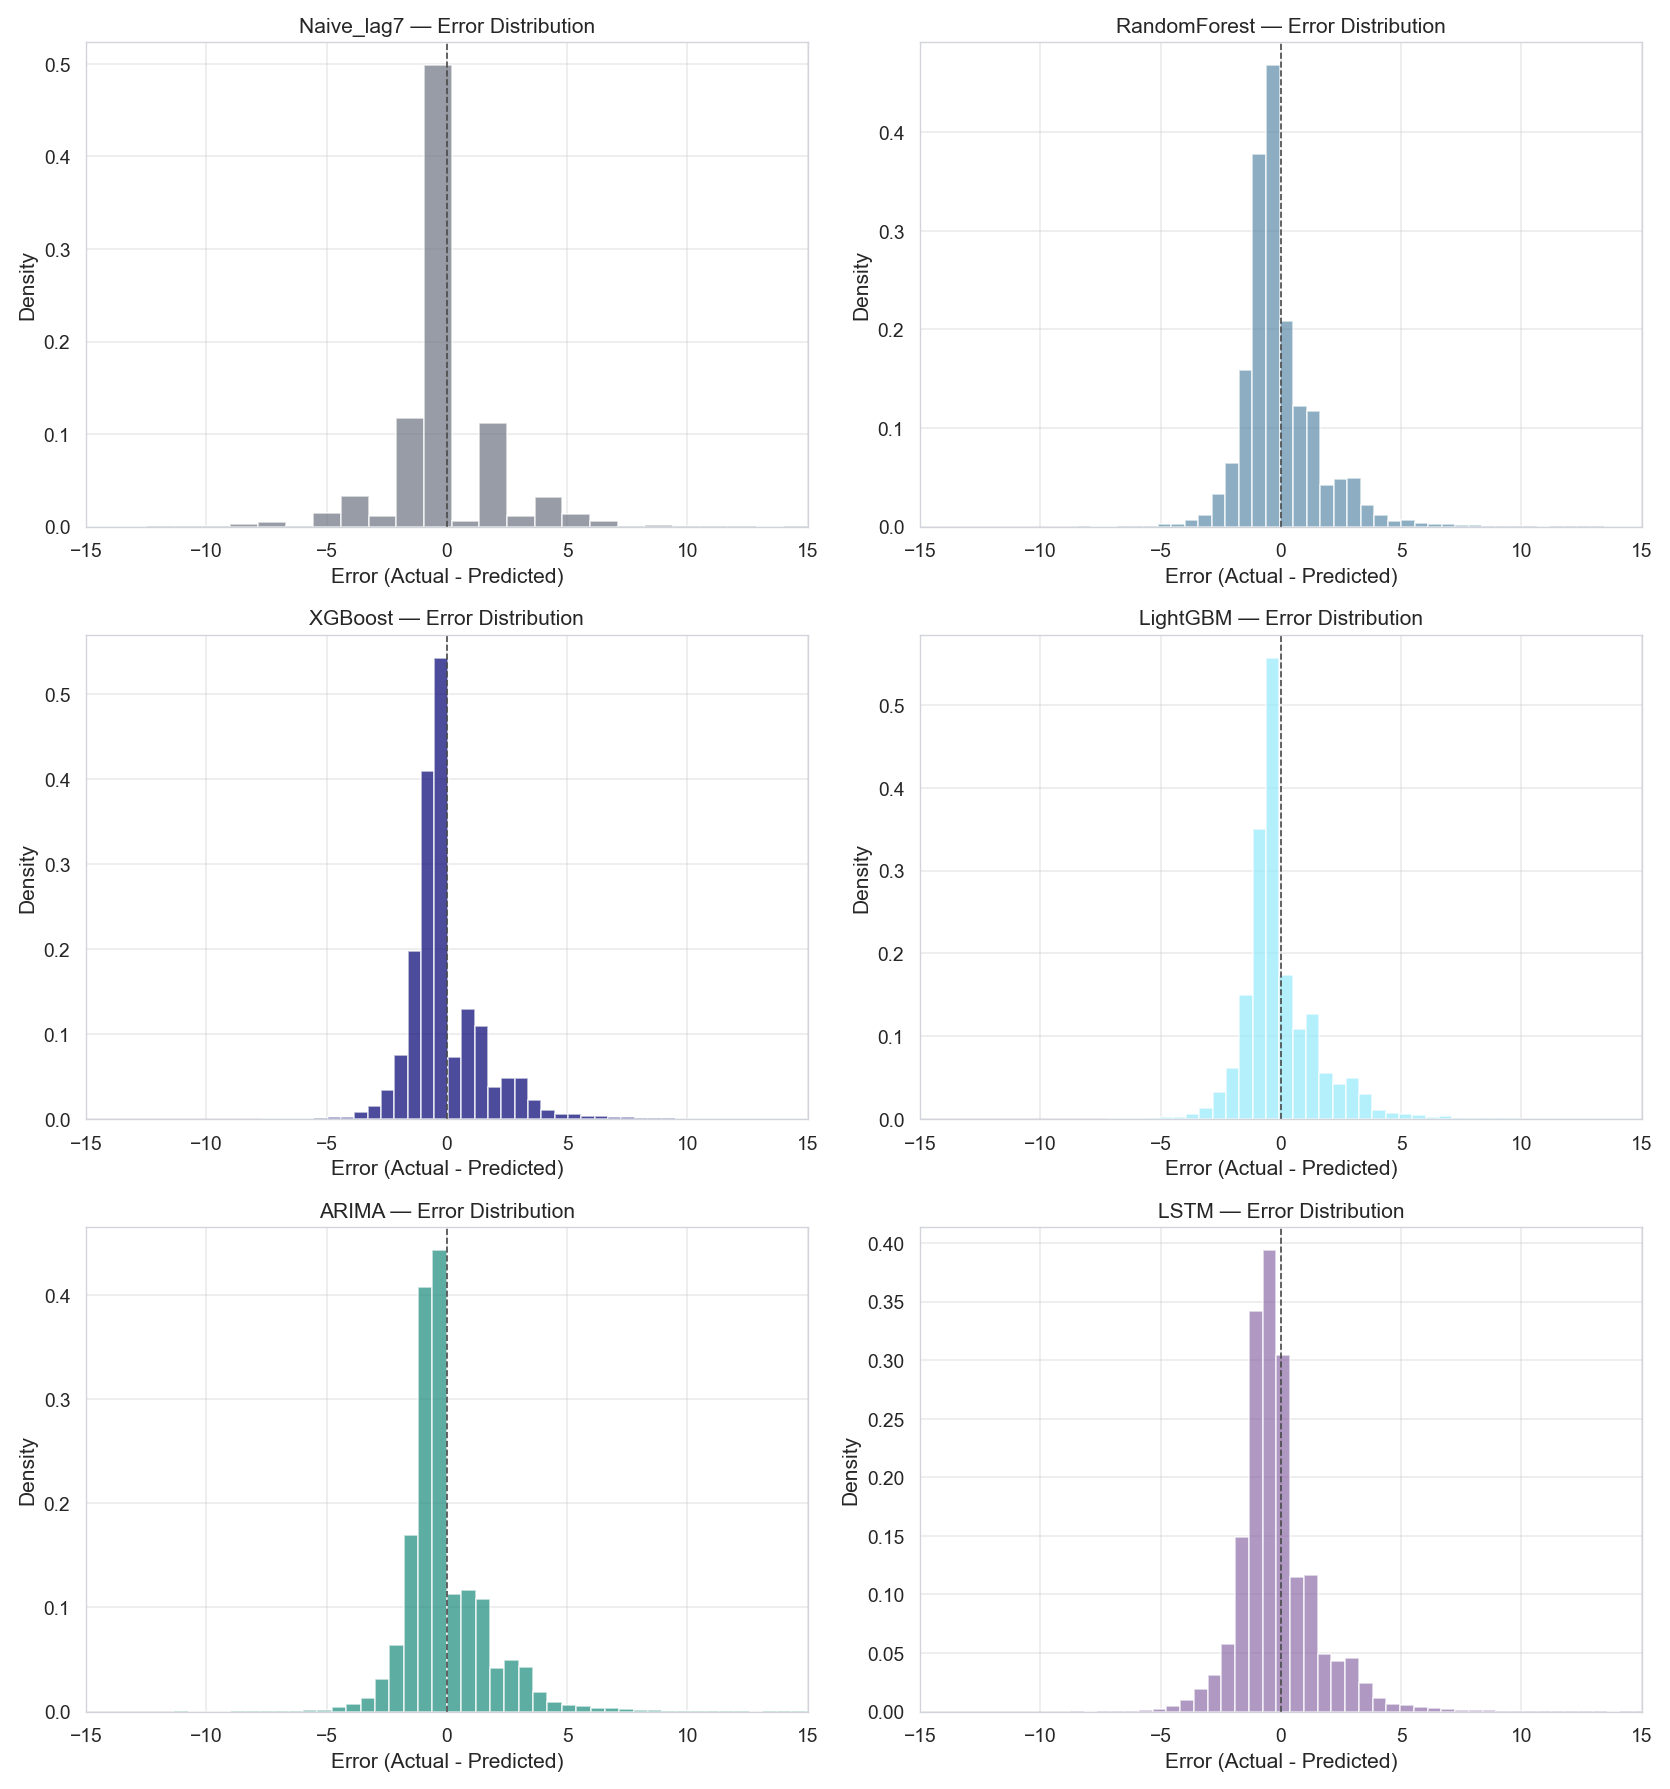
\includegraphics[width=0.85\textwidth]{figures/17_error_distributions.png}
\end{center}
\end{frame}

% ══════════════════════════════════════════════════════════════
% 5. INTERPRETABILITY
% ══════════════════════════════════════════════════════════════
\section{Interpretability}

\begin{frame}{5. Interpretability: SHAP Feature Importance}
\begin{columns}
\begin{column}{0.5\textwidth}
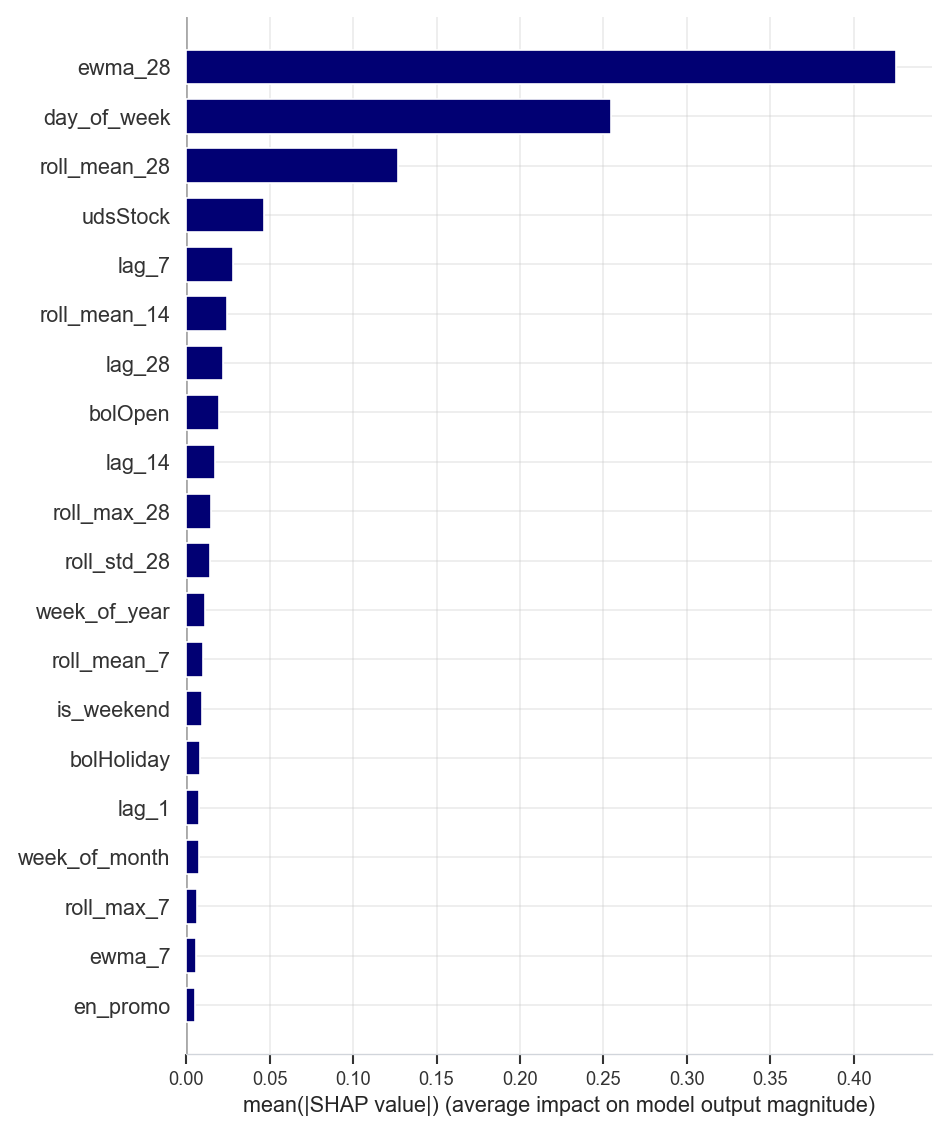
\includegraphics[width=\textwidth]{figures/15_shap_bar.png}
\end{column}
\begin{column}{0.5\textwidth}
\begin{itemize}
    \item 28-day EWMA is the dominant predictor (SHAP = 0.473)
    \item Day of week captures weekly cycle
    \item Rolling statistics and lag features follow
    \item Smoothed demand history drives forecast quality
\end{itemize}
\end{column}
\end{columns}
\end{frame}

% ══════════════════════════════════════════════════════════════
% 6. ECONOMIC IMPACT
% ══════════════════════════════════════════════════════════════
\section{Economic Impact}

\begin{frame}{6. Economic Impact: Safety Stock Cost Analysis}
\begin{block}{Methodology}
$SS_i = z \times RMSE_i \times \sqrt{T_i + L_i}$ \quad\quad $DailyCost_i = 5\% \times price_i \times SS_i$
\end{block}
\vfill
\begin{table}
\centering
\small
\begin{tabular}{lrrr}
\toprule
\textbf{Model} & \textbf{Total SS} & \textbf{Annual Cost} & \textbf{Savings} \\
\midrule
Naive (lag-7) & 12,544 units & \euro11,398,048 & -- \\
Random Forest & 9,105 units & \euro8,310,660 & \euro3,087,388 (27.1\%) \\
XGBoost & 9,090 units & \euro8,307,074 & \euro3,090,974 (27.1\%) \\
LightGBM & 9,133 units & \euro8,341,910 & \euro3,056,137 (26.8\%) \\
\bottomrule
\end{tabular}
\end{table}
\vfill
All three tree-based models save approximately \textbf{\euro3.1 million per year}.
\end{frame}

\begin{frame}{6. Economic Impact: Cost Comparison}
\begin{center}
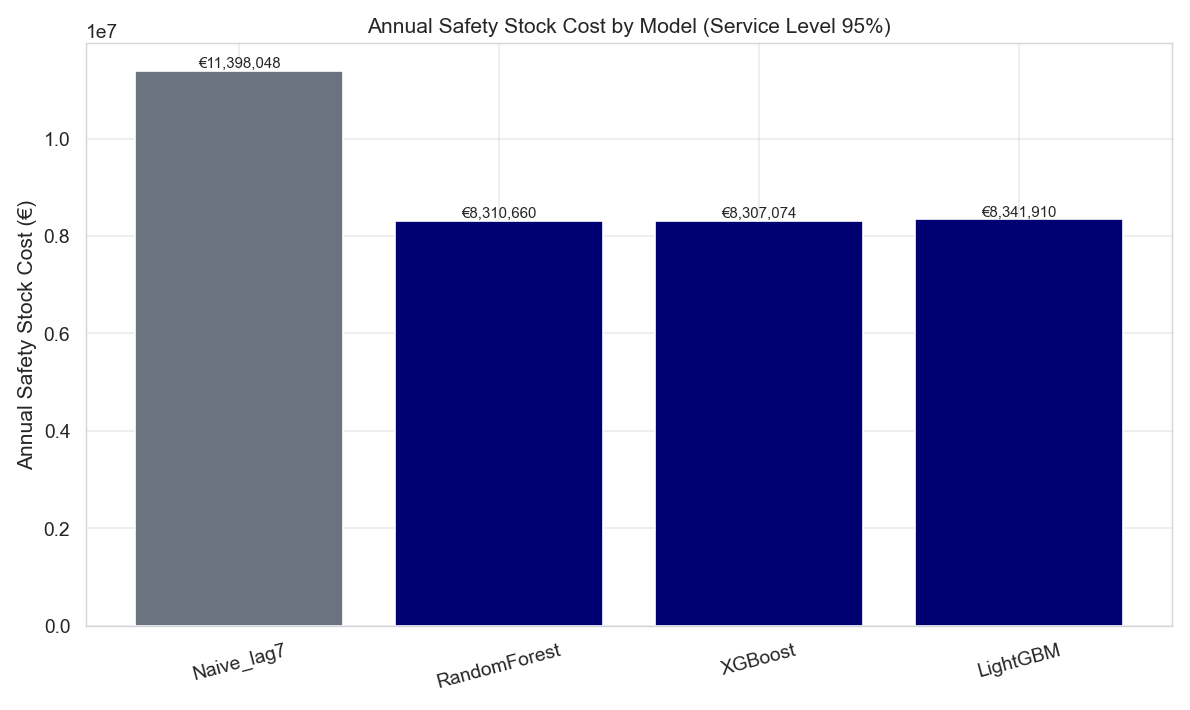
\includegraphics[width=0.75\textwidth]{figures/20_annual_cost_comparison.png}
\end{center}
\end{frame}

\begin{frame}{6. Economic Impact: Sensitivity Analysis}
\begin{center}
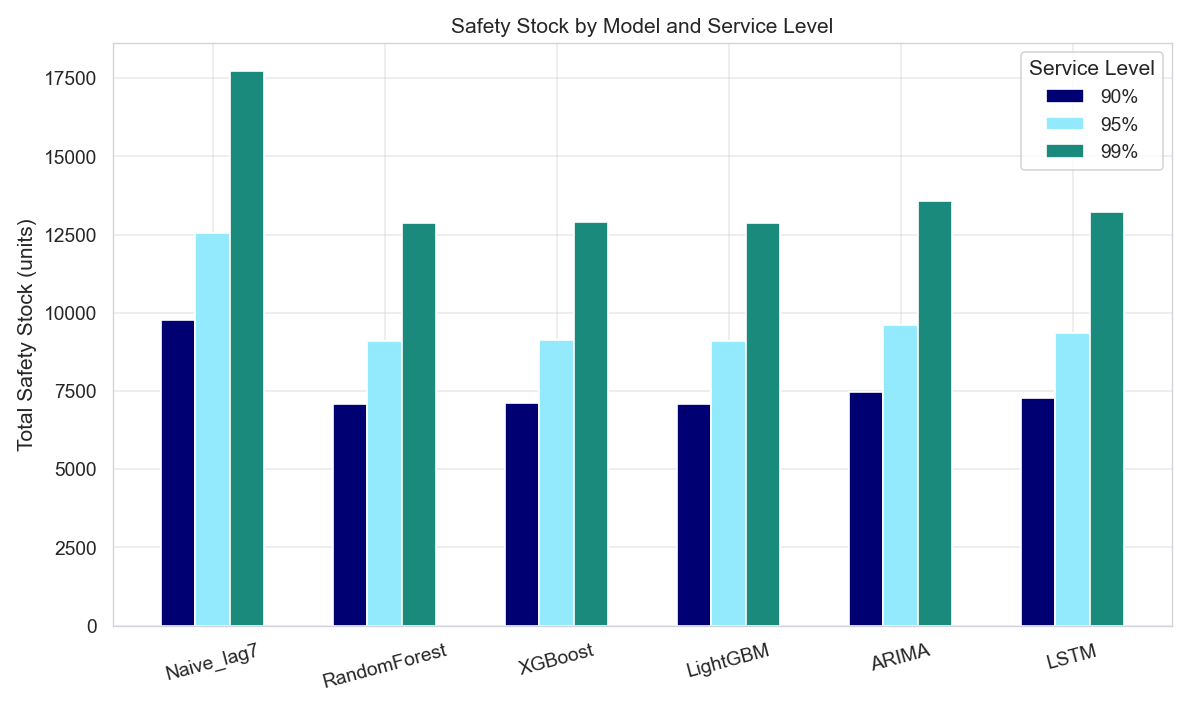
\includegraphics[width=0.75\textwidth]{figures/21_safety_stock_by_service_level.png}
\end{center}
\begin{itemize}
    \item 27\% advantage is consistent across service levels (90\%, 95\%, 99\%)
\end{itemize}
\end{frame}

% ══════════════════════════════════════════════════════════════
% 7. CONCLUSIONS
% ══════════════════════════════════════════════════════════════
\section{Conclusions}

\begin{frame}{7. Conclusions: Key Findings}
\begin{enumerate}
    \item Tree-based ML models reduce forecast error by \textbf{28\%} vs naive baseline
    \item The three tree models (RF, XGBoost, LightGBM) are virtually interchangeable
    \item Feature engineering (EWMA, rolling stats, lags) matters more than model choice
    \item Forecast improvement translates to \textbf{\euro3.1M annual savings} in safety stock costs
    \item Results are robust across service levels and product segments
\end{enumerate}
\end{frame}

\begin{frame}{7. Conclusions: Limitations and Future Work}
\textbf{Limitations:}
\begin{itemize}
    \item Single company, single sector (automotive)
    \item One-day-ahead forecast horizon
    \item No external variables (macroeconomic, competitor data)
\end{itemize}
\vfill
\textbf{Future work:}
\begin{itemize}
    \item Multi-step forecasting over the full protection period
    \item Probabilistic forecasting (prediction intervals)
    \item Automated deployment pipeline for daily operational use
    \item Product-specific forecasting strategies
\end{itemize}
\end{frame}

% ══════════════════════════════════════════════════════════════
% THANK YOU
% ══════════════════════════════════════════════════════════════
{
\setbeamertemplate{headline}{}
\setbeamertemplate{footline}{}
\setbeamercolor{subtitle}{fg=darkblueUOC}
\setbeamercolor{institute}{fg=black}
\setbeamercolor{date}{fg=black}
\begin{frame}[noframenumbering]
\titlepage
\end{frame}
}

\end{document}
